\documentclass[11pt,a4paper]{article}
\usepackage{fullpage}
\usepackage[T1]{fontenc} 
\usepackage[utf8]{inputenc}
\usepackage{amsmath}
\usepackage{amssymb}
\usepackage{float}
\usepackage{tabularx}
\usepackage{multirow}
\usepackage{graphicx}
\usepackage{geometry}
\usepackage[table,dvipsnames]{xcolor}
\usepackage[hidelinks]{hyperref}
\usepackage[polish]{babel}

\def\arraystretch{1.5}
\setlength{\parindent}{0cm}
\setlength{\parskip}{2mm}
\newcolumntype{Y}{>{\centering\arraybackslash}X}

\begin{document}

\title{Metody sztucznej inteligencji 2 \\
\Large{
    Projekt 1. --- Algorytm $k$ najbliższych sąsiadów \\
    Raport
}}
\author{Bartłomiej Dach, Tymon Felski}
\maketitle

Niniejszy dokument zawiera raport z~implementacji algorytmu $k$ najbliższych sąsiadów ($k$-NN, ang. \emph{$k$ nearest neighbors}) oraz~analizę efektywności jego działania dla~dostarczonych danych treningowych.

\section{Algorytm $k$ najbliższych sąsiadów}

Algorytm $k$ najbliższych sąsiadów jest jedną z~wielu metod rozwiązywania \textbf{problemu klasyfikacji}, czyli predykcji wartości zmiennych jakościowych (zwanych również zmiennymi kategorycznymi lub~dyskretnymi) na~podstawie przykładowych \textbf{danych treningowych} \cite[s.~9--10]{hastie2009}.
Klasycznym przykładem tego typu problemu jest klasyfikacja gatunków irysów z~użyciem pomiarów rozmiarów działek kielicha oraz płatków kwiatu. \\

Klasyfikatory oparte na~metodzie $k$ najbliższych sąsiadów operują na~punktach w~przestrzeni $n$-wymiarowej.
Proces klasyfikacji danego punktu $x_0 \in \mathbb{R}^n$ odbywa~się w~następujący sposób:

\begin{enumerate}
    \item Ze~zbioru treningowego wybierane jest $k$ punktów znajdujących~się najbliżej punktu $x_0$ \cite[s.~261]{vapnik1998}.
    \item Jeżeli większość z~wybranych $k$ punktów należy do~jednej klasy, to~punkt wejściowy jest przypisywany do~tej samej klasy.
    \item Potencjalne remisy w~punkcie (2) są~rozstrzygane losowo \cite[s.~463--464]{hastie2009}.
\end{enumerate}

Liczba punktów wybieranych ze~zbioru treningowego (wartość~$k$) stanowi parametr algorytmu.
Jakość działania metody w~dużym stopniu zależy od~odpowiedniego doboru tego parametru dla~danego zadania klasyfikacji \cite[s.~468--470]{hastie2009}. \\

Do~parametrów algorytmu można zaliczyć również metrykę używaną do~obliczania odległości między punktami.
W~zaimplementowanym algorytmie uwzględnione zostały następujące metryki:

\begin{enumerate}
    \item \textbf{odległość euklidesowa}:
    $$ d(x,y) = \sqrt{\sum_{i=1}^n (x_i - y_i)^2} $$
    \item \textbf{odległość taksówkowa (miejska, Manhattan)}:
    $$ d(x,y) = \sum_{i=1}^n |x_i - y_i| $$
    \item \textbf{odległość Czebyszewa (maksimum)}:
    $$ d(x,y) = \max_{i=1,\dots,n} |x_i - y_i| $$
    \item \textbf{odległość Minkowskiego} z~parametrem~$p$, stanowiąca uogólnienie powyższych:
    $$ d(x,y) = \left( \sum_{i=1}^n |x_i - y_i|^p \right)^{1/p} $$
\end{enumerate}

Ponieważ algorytm $k$-NN wymaga zapamiętania całości danych treningowych do~swojego działania, zaliczany jest on do~klasy klasyfikatorów \textbf{opartych na~pamięci} (ang. \emph{memory-based}) \cite[s.~463]{hastie2009}.

\section{Sposób analizy efektywności algorytmu}

Efektywność działania $k$-NN była mierzona z~użyciem dwóch dostarczonych dwuwymiarowych zbiorów danych oraz~zastosowaniem metody kroswalidacji, zalecanej do~doboru parametrów metody \cite[s.~470]{hastie2009}.

\subsection{Kroswalidacja}

\textbf{$k$-krotna kroswalidacja (walidacja krzyżowa, sprawdzian krzyżowy)} to~technika ewaluacji metod klasyfikacji z~użyciem zebranych danych.
W~tej technice zbiór danych treningowych $X$ dzielony~jest losowo na~$k$ rozłącznych podzbiorów $X_1,\dots,X_k$ podobnej liczności. \\

Po~podziale danych wykonywane jest $k$ serii testowych.
W $i$-tej serii testowany klasyfikator jako~dane treningowe otrzymuje zbiór $X \setminus X_i$.
Zadaniem klasyfikatora jest wyznaczenie klas dla~punktów ze~zbioru $X_i$.
Następnie dla~każdego punktu $x_j \in X_i$ następuje porównanie etykiety $y'_j$ wyznaczonej przez testowaną metodę z~etykietą faktyczną $y_j$ \cite[s.~241--243]{hastie2009}. \\

Główną metryką dokładności algorytmu przy~tym porównaniu jest \textbf{proporcja błędnej klasyfikacji}, obliczana wzorem
$$ e_i = \frac{1}{|X_i|} \cdot | \{ y_j \neq y'_j : j = 1,2,\dots,|X_i| \} | $$
Końcowa proporcja błędnej klasyfikacji dla~danej metody jest obliczane poprzez uśrednienie uzyskanych $k$ wyników.

\subsection{Rozważane zbiory treningowe}

Algorytm został przetestowany na~dwuwymiarowych zbiorach {\tt simple} i {\tt three\_gauss}, w~których większość punktów zawiera~się w~kwadracie $[-1,1] \times [-1,1]$.
Oba zbiory mają dość regularną charakterystykę, dzięki czemu możliwe jest również zastosowanie metod statystycznych do~oceny efektywności klasyfikatora $k$-NN.

\subsubsection{Zbiór {\tt simple}}

Zbiór {\tt simple} składa~się z~punktów o~rozkładzie zbliżonym do~jednostajnego wzdłuż obu współrzędnych
Punkty w~tym zbiorze podzielone~są na~dwie klasy wzdłuż prostej o~równaniu $x + y = 0$.
Docelowo klasyfikator powinien więc jak najwierniej odwzorować podział punktów wzdłuż tej prostej.

\subsubsection{Zbiór {\tt three\_gauss}}

Zbiór {\tt three\_gauss} zawiera trzy klasy, częściowo nakładające~się na~siebie.
Każda z~trzech klas charakteryzuje~się rozkładem podobnym do~dwuwymiarowego rozkładu normalnego:

$$ f(\mathbf{x}) = \frac{\exp \left( -\frac{1}{2} (\mathbf{x} - \boldsymbol\mu)^\mathsf{T} \boldsymbol\Sigma^{-1} (\mathbf{x} - \boldsymbol\mu) \right)}{2\pi \sqrt{|\boldsymbol\Sigma|}} $$

Na~podstawie zbioru zawierającego 30~000 punktów wyznaczone zostały przybliżone parametry rozkładów:

\begin{enumerate}
    \item Dla~klasy~1. mamy
    $$
        \boldsymbol\mu_1 \approx \begin{bmatrix} 0.1 \\ 0.5 \end{bmatrix},
        \qquad
        \boldsymbol\Sigma_1 \approx \begin{bmatrix} 0.04 & 0 \\ 0 & 0.04 \end{bmatrix},
    $$
    \item Dla~klasy~2. mamy
    $$
        \boldsymbol\mu_2 \approx \begin{bmatrix} -0.6 \\ 0.2 \end{bmatrix},
        \qquad
        \boldsymbol\Sigma_2 \approx \begin{bmatrix} 0.04 & 0 \\ 0 & 0.0025 \end{bmatrix},
    $$
    \item Dla~klasy~3. mamy
    $$
        \boldsymbol\mu_3 \approx \begin{bmatrix} 0 \\ -0.3 \end{bmatrix},
        \qquad
        \boldsymbol\Sigma_3 \approx \begin{bmatrix} 0.03 & -0.045 \\ -0.045 & 0.16 \end{bmatrix}.
    $$
\end{enumerate}

Używając powyższych parametrów, można podzielić kostkę $[-1, 1] \times [-1, 1]$ na~trzy obszary, obliczając w~każdym jego punkcie \textbf{odległość Mahalanobisa} od~poszczególnych rozkładów wzorem

$$ D_M(\mathbf{x}) = \sqrt{(\mathbf{x} - \boldsymbol\mu)^\mathsf{T} \boldsymbol\Sigma^{-1} (\mathbf{x} - \boldsymbol\mu)} $$

i~przypisując dany punkt do~rozkładu, do~którego jest mu~najbliżej.
Podział ten dla~zbioru {\tt three\_gauss} ukazuje rysunek \ref{fig:gauss-ideal}.

\begin{figure}[H]
    \centering
    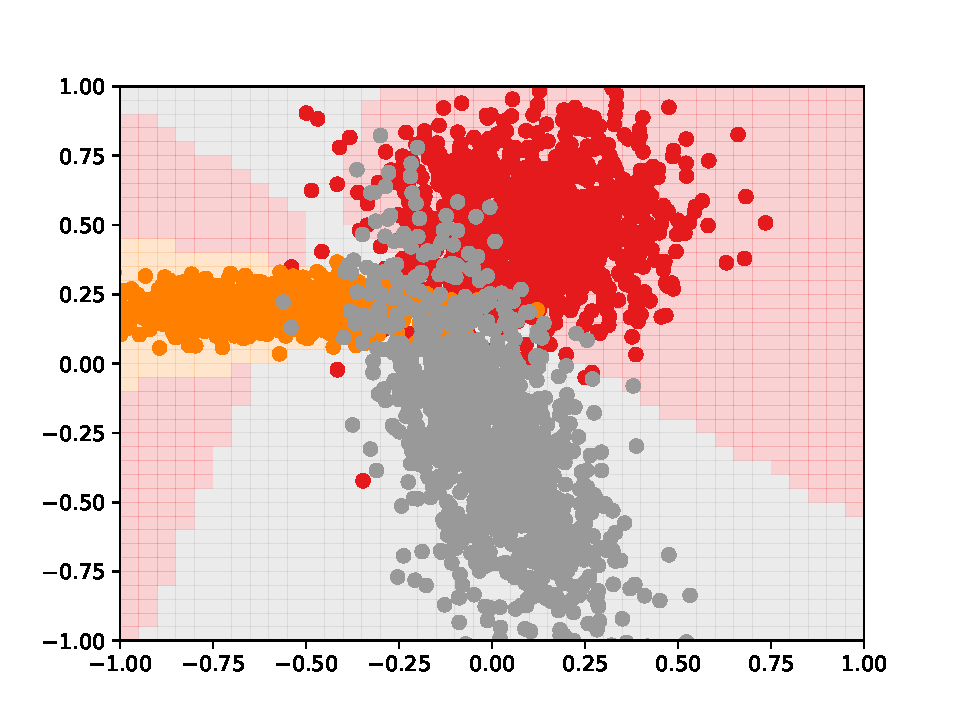
\includegraphics[width=.7\textwidth]{res/gauss-ideal.pdf}
    \caption{Podział obszaru $[-1,1] \times [-1,1]$ na~klasy z~użyciem odległości Mahalanobisa}
    \label{fig:gauss-ideal}
\end{figure}

\section{Wyniki eksperymentów}

Zgodnie z opisem zawartym w poprzednim rozdziale, jakość klasyfikacji przy pomocy algorytmu $k$-NN została przetestowana metodą kroswalidacji przy użyciu dwóch zbiorów treningowych i~różnych wartości parametrów. Zbadano zbiory {\tt simple} oraz {\tt three\_gauss} zawierające odpowiednio $1000$ i $3000$ elementów. Pod uwagę wzięto wartości parametru $k$ ze zbioru $\{1, 3, 5, 7, 9, 11, 13\}$ oraz pięć metryk:
\begin{itemize}
    \setlength\itemsep{-.4em}
    \item odległość taksówkową,
    \item odległość euklidesową,
    \item odległość Czebyszewa,
    \item odległość Minkowskiego z parametrem $p$ wynoszącym $1.5$,
    \item odległość Minkowskiego z parametrem $p$ wynoszącym $3$.
\end{itemize}
Zastosowano pięciokrotną kroswalidację, tzn. dane treningowe zostały losowo podzielone na~$5$~rozłącznych podzbiorów.
We~wszystkich próbach ziarno generatora liczb losowych zostało ustalone, aby~podział był ten~sam dla~wszystkich permutacji wartości parametrów algorytmu.

\subsection{Zbiór {\tt simple}}

\subsubsection{Kroswalidacja}

Wyniki testów jakości klasyfikacji przy pomocy pięciokrotnej kroswalidacji dla zbioru {\tt simple} znajdują się w tabeli poniżej.
Liczby w~tabeli oznaczają średnią proporcję poprawnej klasyfikacji ($1 - \overline{e_i}$).
Kolorem zielonym zaznaczono wynik najlepszy, a kolorem czerwonym~--- najgorszy. Poza najlepszym i najgorszym wynikiem, na pomarańczowo wyróżniono także dwa zestawy parametrów z wynikiem bardzo zbliżonym do najlepszego.

\begin{table}[H]
    \begin{tabularx}{\textwidth}{|c|c|Y|Y|Y|Y|Y|Y|Y|}
        \cline{3-9}
        \multicolumn{2}{c|}{} & \multicolumn{7}{c|}{\textbf{Wartość parametru $k$}} \\
        \cline{3-9}
        \multicolumn{2}{c|}{} & 1 & 3 & 5 & 7 & 9 & 11 & 13 \\
        \hline
        \multirow{5}{*}{\rotatebox[origin=c]{90}{\textbf{Użyta metryka}}}
        & taksówkowa & 0.9850 & \cellcolor{SpringGreen!50}0.9880 &  \cellcolor{YellowOrange!30}0.9870 & 0.9800 & 0.9820 & 0.9800 & 0.9810 \\
        \cline{2-9}
        & euklidesowa & 0.9850 & 0.9860 & 0.9820 & 0.9820 & 0.9830 & 0.9830 & \cellcolor{BrickRed!30}0.9790 \\
        \cline{2-9}
        & Czebyszewa & 0.9830 & 0.9860 & 0.9820 & 0.9810 & 0.9800 & 0.9810 & 0.9820 \\
        \cline{2-9}
        & Minkowskiego ($1.5$) & 0.9850 &  \cellcolor{YellowOrange!30}0.9870 & 0.9840 & 0.9800 & 0.9830 & 0.9810 & 0.9800 \\
        \cline{2-9}
        & Minkowskiego ($3$) & 0.9840 & 0.9850 & 0.9840 & 0.9820 & 0.9800 & 0.9810 & 0.9800 \\
        \hline
    \end{tabularx}
    \caption{Wyniki kroswalidacji algorytmu $k$-NN dla zbioru treningowego {\tt simple}}
    \label{tab:simple-all}
\end{table}

W przypadku powyższych wyników dla zbioru {\tt simple} można zauważyć tendencję osiągania lepszej klasyfikacji dla mniejszych wartości parametrów $k$. Co prawda jest to bardzo mała różnica, ponieważ różnica pomiędzy najlepszym a najgorszym wynikiem nie wynosi nawet $1$ punktu procentowego, jednak jest ona widoczna. Jest to zgodne z przewidywaniami -- dla zbioru, w którym dane są liniowo separowalne, co skutkuje ostrym brzegiem pomiędzy klasami, rozważanie mniejszej liczby sąsiadów pozytywnie wpływa na ostateczny wynik, ponieważ nie rozmywa brzegu. Najlepiej wypadła tutaj klasyfikacja algorytmem $k$-NN dla $k=3$ i z metryką taksówkową, jednak takie samo wywołanie dla $k=5$ oraz wywołanie z $k=3$ i metryką Minkowskiego przy $p=1.5$ dały bardzo zbliżone wyniki. Równomierny rozkład punktów w~obszarze niweluje różnice w~wynikach spowodowane wyborem metryki.
\\

Po ustaleniu najkorzystniejszych wartości parametrów algorytmu $k$-NN dla powyższego zbioru, zdecydowano się zbadać cały obszar $[-1,1] \times [-1,1]$ z gęstością próbkowania $\delta = 0.05$ i ustalić przynależność środkowych punktów każdego z kwadratów o boku~$\delta$, zawartych w tym obszarze, do jednej z klas zbioru treningowego. Poniższy wykres jest graficzną reprezentacją otrzymanych wyników dla $k = 3$ oraz metryki będącej odległością taksówkową.

\begin{figure}[H]
  \centering
  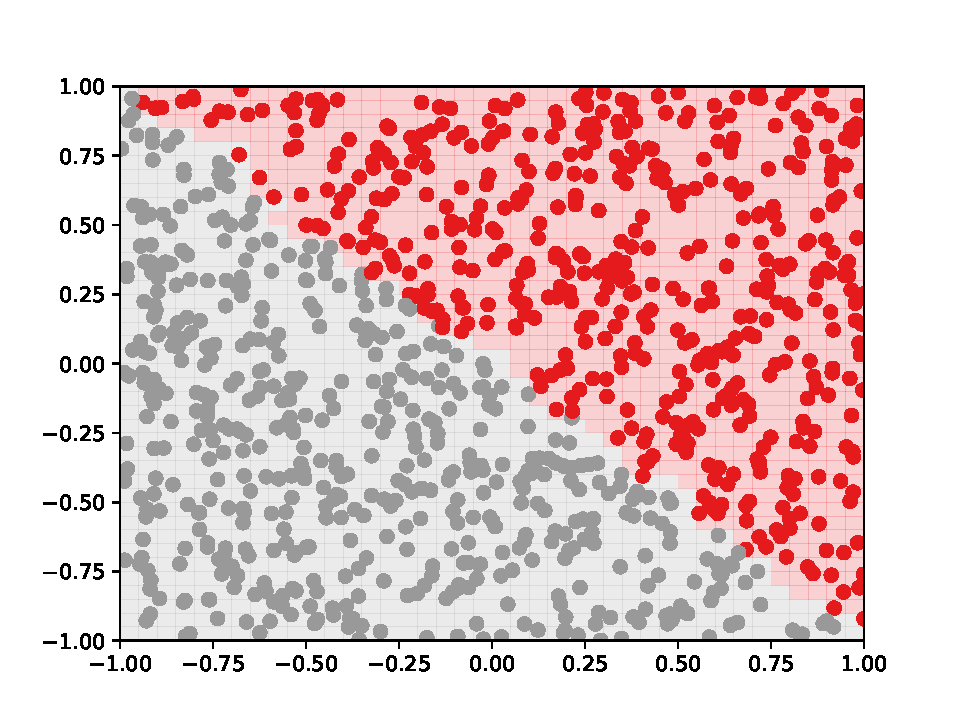
\includegraphics[width=.7\textwidth]{res/simple-manhattan-3.pdf}
  \caption{Klasyfikacja punktów z obszaru $[-1,1] \times [-1,1]$ dla $k = 3$ i odległości taksówkowej}
  \label{fig:simple-manhattan-3}
\end{figure}

\newpage

Dla kontrastu, podobną analizę przeprowadzono dla parametrów, które zapewniły najgorszą klasyfikację, czyli dla $k=13$ i odległości euklidesowej.

\begin{figure}[H]
  \centering
  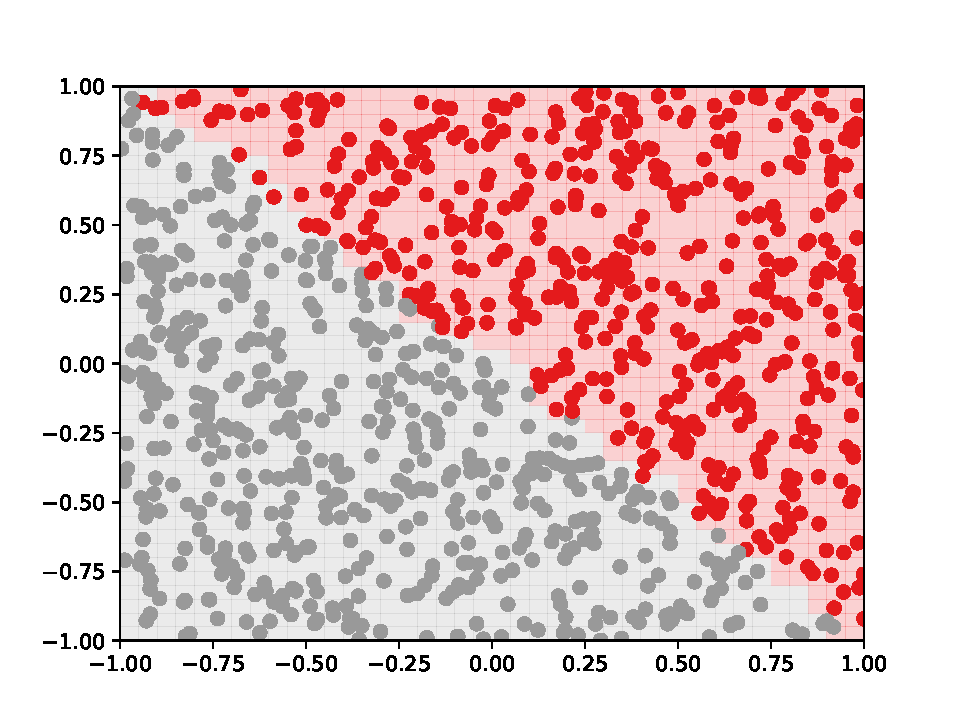
\includegraphics[width=.7\textwidth]{res/simple-euclidean-13.pdf}
  \caption{Klasyfikacja punktów z obszaru $[-1,1] \times [-1,1]$ dla $k = 13$ i odległości euklidesowej}
  \label{fig:simple-euclidean-13}
\end{figure}

Zamieszczone powyżej wykresy \ref{fig:simple-manhattan-3} oraz \ref{fig:simple-euclidean-13} potwierdzają opisane wcześniej przypuszczenia. Rozważanie aż $13$ sąsiadów powoduje, że brzeg punktów ze zbioru nie jest poprawnie wyznaczony. Zjawisko rozmycia jest szczególnie widoczne w okolicy punktu $(-0.6, 0.7)$, w drugiej ćwiartce wykresu. Wokół punktów z klasy czerwonej, które znajdują się na brzegu, znajduje się więcej punktów z klasy szarej, co skutkuje zaklasyfikowaniem obszaru jako szary.

\subsubsection{Analiza powstałych obszarów}

Dla~wyznaczonego w~procesie kroswalidacji parametru~$k=3$ przetestowano wpływ wyboru metryki na~odwzorowanie kształtu brzegów między obszarami wyznaczonymi przez~klasyfikator.
Po~podziale obszaru $[-1,1] \times [-1,1]$ dokonano próbkowania klasyfikatora dla~równoodległych punktów z~interwałem $\delta = 0.05$ i~porównania wynikowych etykiet z~idealnymi.
Wyniki tego eksperymentu znajdują~się w~tabeli \ref{tbl:shape-simple}.

\begin{table}[H]
    \centering
    \begin{tabularx}{0.6\textwidth}{|c|Y|}
        \hline
        \textbf{Użyta metryka} & \textbf{Jakość odwzorowania brzegu} \\
        \hline
        taksówkowa & \cellcolor{BrickRed!30}0.9786 \\
        \hline
        Minkowskiego ($p = 1.5$) & 0.9798 \\
        \hline
        euklidesowa & 0.9810 \\
        \hline
        Minkowskiego ($p = 3$) & \cellcolor{YellowOrange!30}0.9827 \\
        \hline
        Czebyszewa & \cellcolor{SpringGreen!50}0.9833 \\
        \hline
    \end{tabularx}
    \caption{Wyniki porównania odwzorowania brzegów między zbiorami przez~algorytm $k$-NN z~odwzorowaniem dokładnym dla~zbioru {\tt simple}}
    \label{tbl:shape-simple}
\end{table}

Różnice między poszczególnymi metrykami nie~są znaczne (rozstęp $0.5$ punkta procentowego różnicy), lecz~najlepszym wynikiem wykazała~się metryka Czebyszewa.

\subsection{Zbiór {\tt three\_gauss}}

\subsubsection{Kroswalidacja}

Pięciokrotną kroswalidację badanego klasyfikatora przeprowadzono także dla zbioru {\tt three\_gauss}. Jej wyniki znajdują się w tabeli poniżej. Komórki tabeli wyróżnione kolorami: zielonym, czerwonym i pomarańczowym mają tutaj takie same znaczenia.

\begin{table}[H]
    \begin{tabularx}{\textwidth}{|c|c|Y|Y|Y|Y|Y|Y|Y|}
        \cline{3-9}
        \multicolumn{2}{c|}{} & \multicolumn{7}{c|}{\textbf{Wartość parametru $k$}} \\
        \cline{3-9}
        \multicolumn{2}{c|}{} & 1 & 3 & 5 & 7 & 9 & 11 & 13 \\
        \hline
        \multirow{5}{*}{\rotatebox[origin=c]{90}{\textbf{Użyta metryka}}}
        & taksówkowa & \cellcolor{BrickRed!30}0.9053 & 0.9233 & 0.9257 & 0.9283 & \cellcolor{SpringGreen!50}0.9333 & 0.9280 & 0.9290 \\
        \cline{2-9}
        & euklidesowa & 0.9073 & 0.9220 & 0.9230 & 0.9303 & 0.9290 & 0.9290 & 0.9267 \\
        \cline{2-9}
        & Czebyszewa & 0.9113 & 0.9213 & 0.9217 & 0.9253 & 0.9277 & \cellcolor{YellowOrange!30}0.9307 & 0.9300 \\
        \cline{2-9}
        & Minkowskiego ($1.5$) & 0.9070 & 0.9237 & 0.9253 & 0.9290 & \cellcolor{YellowOrange!30}0.9307 & 0.9280 & 0.9263 \\
        \cline{2-9}
        & Minkowskiego ($3$) & 0.9090 & 0.9210 & 0.9230 & 0.9300 & 0.9297 & 0.9297 & 0.9297 \\
        \hline
    \end{tabularx}
    \caption{Wyniki kroswalidacji algorytmu $k$-NN dla zbioru treningowego {\tt three\_gauss}}
    \label{tab:simple-all}
\end{table}

Jak już zostało to wcześniej opisane, klasy punktów w zbiorze {\tt three\_gauss} częściowo na siebie nachodzą; ponadto mamy w~nim do~czynienia z~tzw. obserwacjami odstającymi, czyli punktami z~klasy, które znajdują~się daleko od~pozostałych.
Wybór większego parametru $k$ pozwala na~zniwelowanie wpływu obserwacji odstających na~działanie algorytmu, co~demonstrują dane doświadczalne.
Lepsze wyniki klasyfikacji można dostrzec w prawej części tabeli. Najlepiej wypadło tutaj wywołanie dla $k=9$ z metryką taksówkową, jednak niewiele gorszy wynik można osiągnąć dla takiej samej wartości $k$ z metryką Minkowskiego dla $p=9$ lub dla $k=11$ i odległości Czebyszewa. Różnica pomiędzy najgorszym a najlepszym wynikiem wynosi w przypadku zbioru {\tt three\_gauss} już aż prawie 3 punkty procentowe.\\ % TODO: bardziej skomentować metryki

Dla wyróżnionych parametrów algorytmu $k$-NN podczas klasyfikacji zbioru {\tt three\_gauss} przeprowadzono analogiczną analizę, jak w przypadku zbioru {\tt simple}. Punkty z obszaru $[-1,1] \times [-1,1]$ z gęstością próbkowania $\delta = 0.05$ zostały sklasyfikowane, w celu wizualizacji przyporządkowania. Poniższy wykres zawiera wyniki uzyskane dla wywołania algorytmu $k$-NN dla $k=9$ i odległości taksówkowej.

\begin{figure}[H]
  \centering
  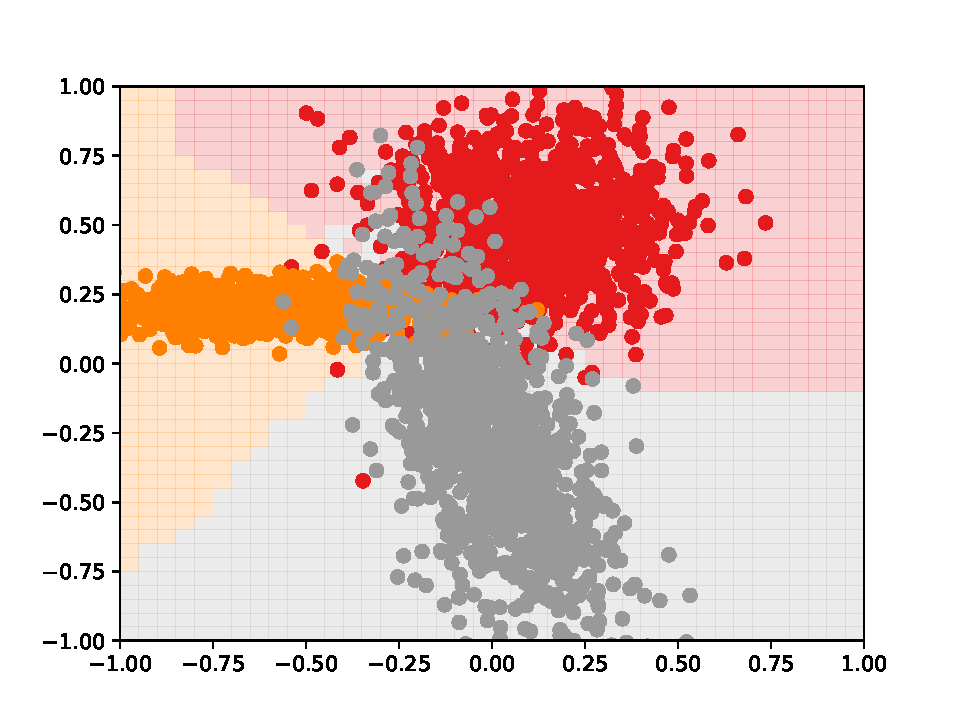
\includegraphics[width=.7\textwidth]{res/gauss-manhattan-9.pdf}
  \caption{Klasyfikacja punktów z obszaru $[-1,1] \times [-1,1]$ dla $k = 9$ i odległości taksówkowej}
  \label{fig:gauss-manhattan-9}
\end{figure}

\newpage

Podobnie jak w poprzednim podrozdziale, dla zbioru {\tt three\_gauss} również zwizualizowano wynik działania algorytmu $k$-NN dla najgorszego zestawu parametrów, czyli $k=1$ i odległości taksówkowej. Przedstawia to poniższy wykres.

\begin{figure}[H]
  \centering
  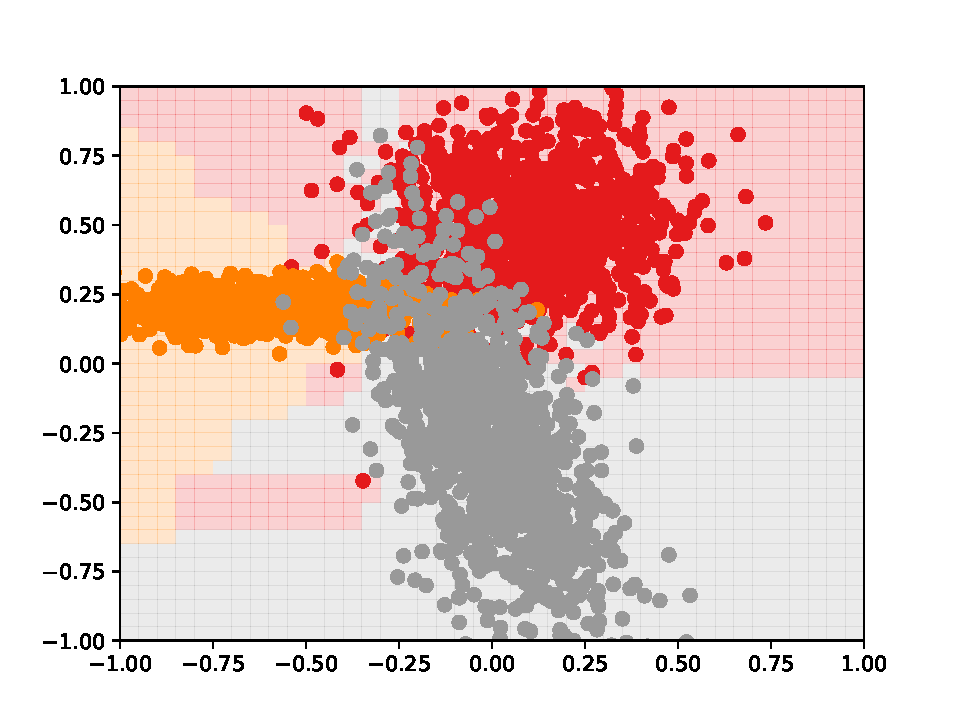
\includegraphics[width=.7\textwidth]{res/gauss-manhattan-1.pdf}
  \caption{Klasyfikacja punktów z obszaru $[-1,1] \times [-1,1]$ dla $k = 1$ i odległości taksówkowej}
  \label{fig:gauss-manhattan-1}
\end{figure}

Zamieszczone powyżej wykresy \ref{fig:gauss-manhattan-9} oraz \ref{fig:gauss-manhattan-1} pokazują znaczenie poprawnego dobrania wartości parametru $k$ dla zbioru o takiej charakterystyce. Rozważanie większej liczby sąsiadów (w tym przypadku dziewięciu) powoduje, że punkty z danej klasy znajdujące się daleko od pozostałych nie~wpływają na~klasyfikację w swojej okolicy, jeżeli zdecydowana większość sąsiadów należy do innej klasy. Dobrym przykładem tego zjawiska jest punkt z klasy czerwonej znajdujący się w okolicy punktu $(-0.3, -0.45)$. Dla~$k=9$ został on pominięty i znajduje się w obszarze należącym do klasy szarej. W przypadku klasyfikacji z $k=1$ punkt ten znacznie wpłynął na ostateczny wynik i~spowodował przyporządkowanie sporego obszaru trzeciej ćwiartki wykresu do~swojej klasy.

\subsubsection{Analiza powstałych obszarów}

Analogicznie jak w~przypadku zbioru {\tt simple}, kształt obszarów wyznaczonych przez $k$-NN porównano z~wzorcowym (w~tym przypadku jest to~podział wyznaczony przez odległość Mahalanobisa, ukazany na~rys. \ref{fig:gauss-ideal}).
Wyniki tego eksperymentu znajdują~się w~tabeli \ref{tbl:shape-gauss}.

\begin{table}[H]
    \centering
    \begin{tabularx}{0.6\textwidth}{|c|Y|}
        \hline
        \textbf{Użyta metryka} & \textbf{Jakość odwzorowania brzegu} \\
        \hline
        taksówkowa & \cellcolor{BrickRed!30}0.7829 \\
        \hline
        Minkowskiego ($p = 1.5$) & 0.7948 \\
        \hline
        euklidesowa & 0.7995 \\
        \hline
        Minkowskiego ($p = 3$) & \cellcolor{YellowOrange!30}0.8061 \\
        \hline
        Czebyszewa & \cellcolor{SpringGreen!50}0.8126 \\
        \hline
    \end{tabularx}
    \caption{Wyniki porównania odwzorowania brzegów między zbiorami przez~algorytm $k$-NN z~odwzorowaniem wyznaczonym przez~metrykę Mahalanobisa dla~zbioru {\tt three\_gauss}}
    \label{tbl:shape-gauss}
\end{table}

Jakość odwzorowania w~tym przypadku znacząco spada, ponieważ podział przedstawiony na~wykresie \ref{fig:gauss-ideal} nie~jest intuicyjny z~geometrycznego punktu widzenia.
Algorytm $k$-NN w~dużej mierze opiera~się na~miarach w~celu wyznaczenia sąsiedztwa, więc szczególnie w~drugiej ćwiartce układu współrzędnych (blisko klasy 2, oznaczonej na~rysunkach kolorem pomarańczowym) rozbieżności są duże.
Natomiast i~w~tym przypadku zauważalny jest~wzrost jakości odwzorowania wraz~z~wzrostem parametru~$p$ w~normie Minkowskiego.

\section{Wnioski}

Algorytm $k$ najbliższych sąsiadów jest jednym z~najprostszych klasyfikatorów pod~względem zasady działania.
Testy z~dostarczonymi zbiorami pokazały jednak, że~jest on~w~stanie osiągać bardzo dobre wyniki dla~danych o~odpowiedniej regularności.
Dużym minusem algorytmu jest jednak konieczność zapamiętania całego zbioru treningowego, co~jest w~przypadku dużych ilości danych źródłem problemów zarówno pamięciowych, jak i~wydajnościowych. \\

Z~przeprowadzonych eksperymentów wynika, że~odpowiedni dobór parametrów klasyfikatora stanowi kluczową rolę w~jego dokładnym działaniu.
Przy~doborze parametru $k$ należy brać pod~uwagę czynniki takie, jak separowalność klas, zaszumienie danych oraz~występowanie obserwacji odstających, zaś wybór metryki ma~znaczący wpływ na~kształty obszarów, na~które klasyfikator dzieli przestrzeń $\mathbb{R}^n$.

\begin{thebibliography}{9}

    \bibitem{hastie2009}
        T. Hastie,
        R. Tibshirani,
        J. Friedman,
        \emph{The Elements of Statistical Learning: Data Mining, Inference, and Prediction}.
        Nowy Jork: Springer-Verlag,
        2009.
        [Online] \\
        Dostępne: \url{https://web.stanford.edu/~hastie/ElemStatLearn/}.
        [Dostęp 26~lutego 2018]

    \bibitem{vapnik1998}
        V.N. Vapnik,
        \emph{Statistical learning theory}.
        Nowy Jork: John Wiley and Sons,
        1998.

\end{thebibliography}

\end{document} % TODO: sformatować całość, żeby nie było jakichś pustych stron (resize obrazków?)